\documentclass[tikz,border=10pt]{standalone}
\usepackage{tikz}
\usetikzlibrary{arrows.meta}

\begin{document}
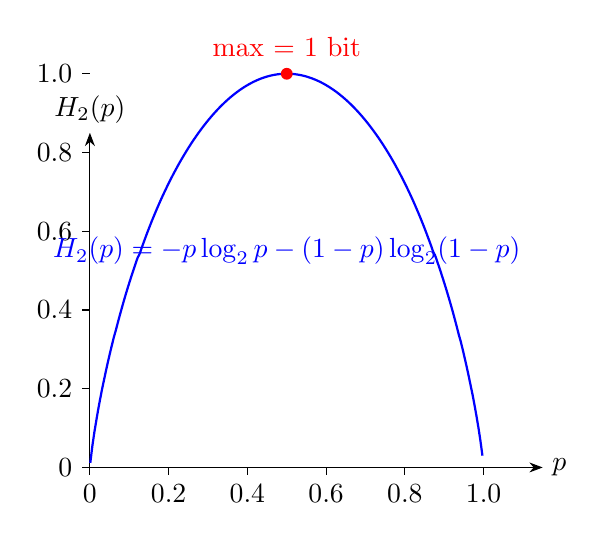
\begin{tikzpicture}[>=Stealth, scale=5]
\draw[->] (0,0) -- (1.15,0) node[right] {$p$};
\draw[->] (0,0) -- (0,0.85) node[above] {$H_2(p)$};
\foreach \x in {0,0.2,0.4,0.6,0.8,1.0} {
    \draw (\x,0) -- (\x,-0.02) node[below] {\x};
}
\foreach \y in {0,0.2,0.4,0.6,0.8,1.0} {
    \draw (0,\y) -- (-0.02,\y) node[left] {\y};
}
\draw[thick, blue, domain=0.001:0.999, samples=200] 
    plot (\x, {-\x*ln(\x)/ln(2) - (1-\x)*ln(1-\x)/ln(2)});
\node[blue] at (0.5,0.55) {$H_2(p) = -p\log_2 p - (1-p)\log_2(1-p)$};
\fill[red] (0.5,1) circle (0.015);
\node[red, above] at (0.5,1.02) {max = 1 bit};
\end{tikzpicture}
\end{document}
